\documentclass[a4paper, 12pt]{article}

\usepackage[utf8]{inputenc}
\usepackage{latexsym,amsfonts,amssymb,amsthm,amsmath}
\usepackage{setspace}
\usepackage{physics}
\usepackage{graphicx}
\usepackage{newtxtext}
\usepackage{extsizes}
\setlength{\parindent}{0in}
\setlength{\oddsidemargin}{0in}
\setlength{\textwidth}{6.5in}
\setlength{\textheight}{8.8in}
\setlength{\topmargin}{0in}
\setlength{\headheight}{8pt}

\onehalfspacing


\title{
  \vspace{-1.5cm}
  \textbf{Important distributions in Statistics}
  \vspace{-1.5cm}
}
\date{}

\begin{document}

\maketitle

In this lecture, we will focus on certain distributions that have wide application in statistics. These are:

\begin{itemize}
  \item \textbf{Normal distribution} (Inference about means - known $\sigma$)
  \item \textbf{Chi-squared distribution} (Inference about variance \& categorical data - simple varaince, counts)
  \item \textbf{Student or $t$-distribution} (Inference about means - unknown $\sigma$)
  \item \textbf{Fisher $F$-distribution} (Comparing two variances or multiple means - two sample variances)
\end{itemize}


\section{Normal distribution}

A random variable $X$ has a normal distribution with parameters $\mu$ and $\sigma^2$, denoted as $X \sim N(\mu, \sigma^2)$, if its probability density function is given by:


\[ p(x) = \frac{1}{\sqrt{2\pi \sigma^2}} e^{-\frac{(x-\mu)^2}{2\sigma^2}} \]

\begin{itemize}
  \item [] $\mu = EX$ is mathematical expectation
  \item [] $\sigma^2 = DX$ is variance of $X$
\end{itemize}


For the density graph of an arbitrary normal distribution, it can be shown that the following holds for the areas under the curve:

\begin{itemize}
  \item About $68.3\%$ of the area lies within the interval $(\mu - \sigma, \mu + \sigma)$
  \item About $98.5\%$ of the area lies within the interval $(\mu - 2\sigma, \mu + 2\sigma)$
  \item About $99.57\%$ of the area lies within the interval $(\mu - 3\sigma, \mu + 3\sigma)$
\end{itemize}

Practically, the area under the curve outside the interval $(\mu - 4\sigma, \mu + 4\sigma)$ is 0. This means that although the graph extends to infinity, beyond the interval $(\mu - 4\sigma, \mu + 4\sigma)$ it is so close to the x-axis that the area between the graph of $p(x)$ and the x-axis is 0.

\begin{figure}[h!]
  \centering
  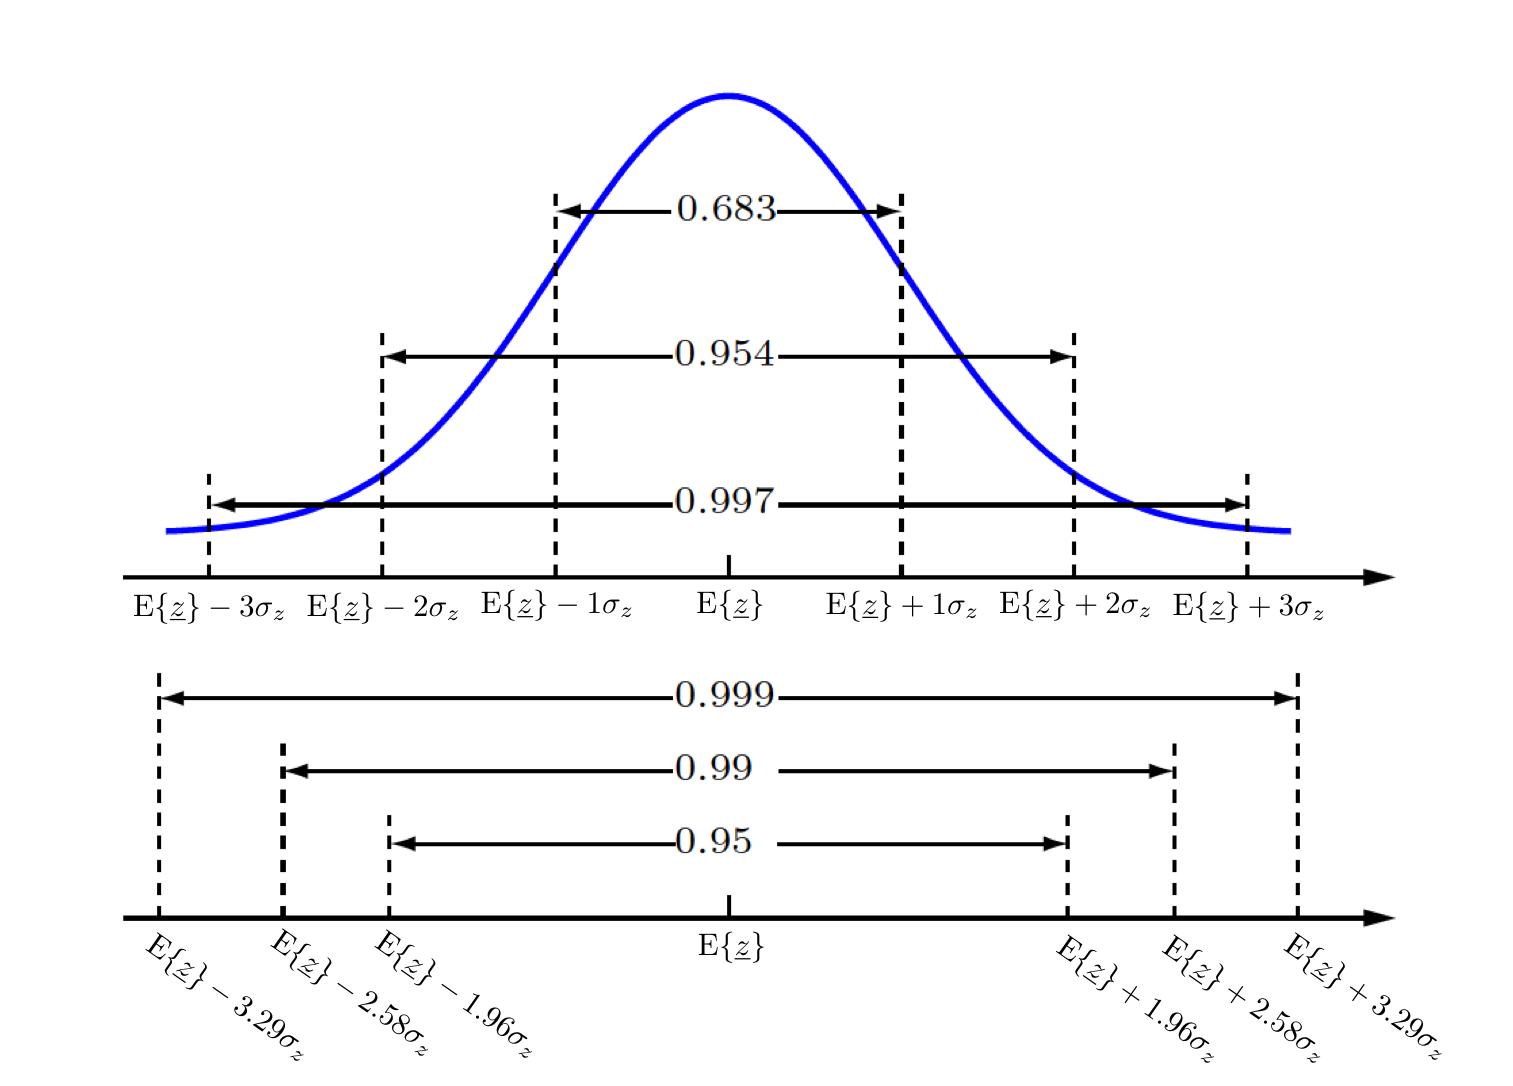
\includegraphics[width=0.7\textwidth]{normal-d.png}
  \caption{Normal distribution}
  \label{normal-distr}
  
\end{figure}

\subsection{Tables for normal distribution}

For the standard normal distribution, there are tables. In them, the values of the distribution function are tabulated, and for a given value a one can look up the value of $\Phi(a) = P\{Z < a\}$, i.e., the area under the density curve over the interval from minus infinity to a.\\

From the tables, the value $\Phi(a)$ can be found for $a \in (-4, 4)$. Namely, for this distribution $\mu = 0$ and $\sigma = 1$, so the area under the curve outside the interval $(\mu - 4\sigma, \mu + 4\sigma) = (-4, 4)$ is 0, i.e., the probability that the random variable will take a value outside this interval is 0. Therefore, if $a \leq-4$ then $\Phi(a) = 0$, and if $a \geq 4$ then $\Phi(a) = 1$.

\begin{figure}[h!]
  \centering
  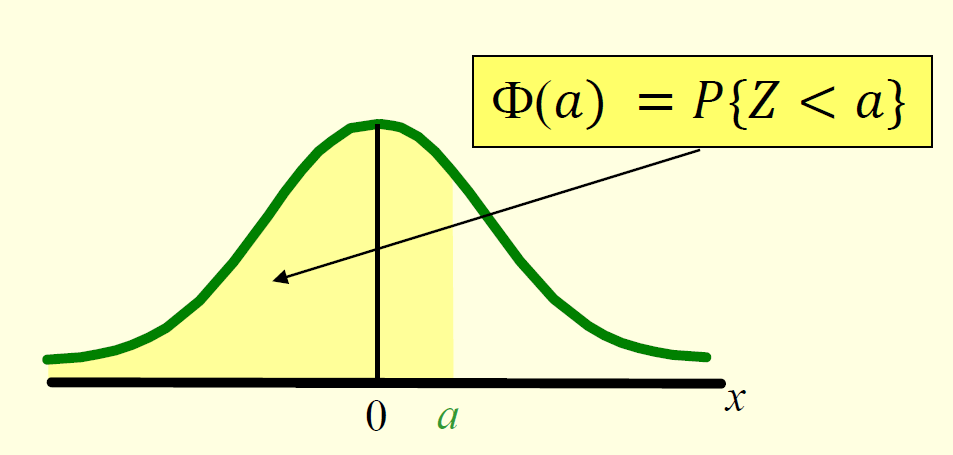
\includegraphics[width=0.6\textwidth]{phi.png}
  \caption{}
  \label{fig:phi}
  
\end{figure}

From the tables of negatives and positives the following expression can be calculated directly:

\[ P\{ Z < 1.48 \} = 0.93056 \]
\[ P\{ Z < -265 \} = 0.00402 \]

If we need to read from the table the probability that any other random variable $X \sim N(\mu, \sigma^2)$ takes a value from a certain interval, we must first transform that variable into a random variable $Z \sim N(0,1)$.\\

As known from before, the transformation is done by subtracting the mean of $X$ and dividing by the square root of its variance (which is called the standard deviation):

\[ Z = \frac{X-\mu}{\sigma} \]

For a given value $x_0$, the value $z_0 = \frac{x_0 - \mu}{\sigma}$ indicates how many standard deviations $x_0$ deviates from the mean $\mu$.\\

For example, if $X$ has a normal distribution with mean 100 and standard deviation 50, the $z$-value for $x = 200$ is:

\[ z = \frac{x-\mu}{\sigma} = \frac{200-100}{50} = 2.0 \]

That means that $x = 200$ is two standard deviations from expectation $\mu = 100$.

\subsection{Procedure for determining probabilities in a normal distribution}

Let $X \sim N(\mu, \sigma^2)$. To calculate $P\{a < X < b\}$, first transform $X$ into $Z \sim N(0,1)$, and then read the values from the standard normal distribution table.\\

With transformation the following is obtained:

\newpage
\begin{align*}
  P\{ a < X < b \} 
  &= P \Bigg\{ \frac{a-\mu}{\sigma} < \frac{X-\mu}{\sigma} < \frac{b-\mu}{\sigma} \Bigg\} \\
  &= P \Bigg\{ \frac{a-\mu}{\sigma} < Z < \frac{b-\mu}{\sigma} \Bigg\} \\
  &= F_Z \Bigg( \frac{b-\mu}{\sigma} \Bigg) - F_Z \Bigg( \frac{a-\mu}{\sigma} \Bigg) \\
  &= \Phi \Bigg( \frac{b-\mu}{\sigma} \Bigg) - \Phi \Bigg( \frac{a-\mu}{\sigma} \Bigg)
\end{align*}


\begin{figure}[h!]
  \centering
  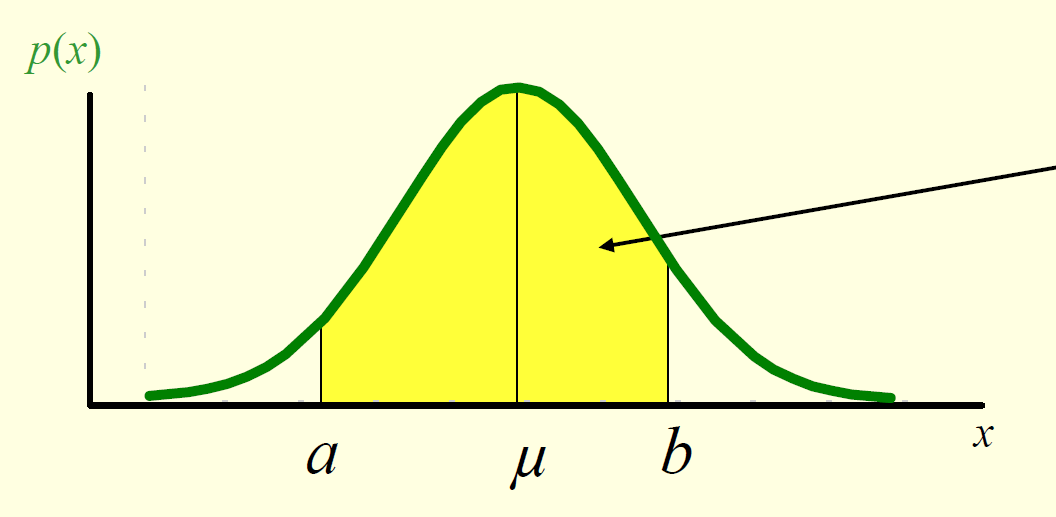
\includegraphics[width=0.6\textwidth]{phib-phia.png}
  \caption{}
  \label{fig:phib-phia}
\end{figure}

Now the values $\displaystyle\Phi \Bigg( \frac{b-\mu}{\sigma} \Bigg)$ and $\displaystyle\Phi \Bigg( \frac{a-\mu}{\sigma} \Bigg)$ are read from the tables for standard normal distribution.


\newpage
\subsubsection*{Example 1}

For example, let $X$ be a normally distributed random variable with mean 8 and variance 25 ($X \sim N(8, 25)$), and we want to determine $P\{X < 8.6\}$.

\textbf{Solution.}

First, transform $X$ to $Z$:

\[ P\{ X < 8.6 \} =  P \Bigg\{ \frac{X-\mu}{\sigma} < \frac{8.6-8.0}{5.0}\Bigg\} = P\{ Z < 0.12 \} = \Phi(0.12) = 0.54776 \]



\begin{figure}[h!]
  \centering
  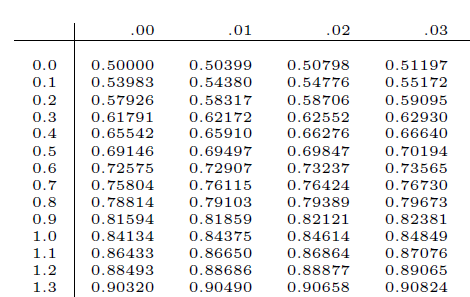
\includegraphics[width=0.6\textwidth]{image.png}
  \caption{}
  \label{fig:example_1}
\end{figure}

\subsection{Determining $z$ value}

How do we determine the value of $z$ for which $\Phi(z) = 0.2$ for the random variable $Z \sim N(0,1)$?
\begin{itemize}
  
\item In the table of $\Phi$ values, we look for the value 0.2 (or the closest to it) and then read for which $z$ value $\Phi(z) = 0.2$.
\item From the table, we find $z = -0.84$.



\begin{figure}[h]
  \centering
  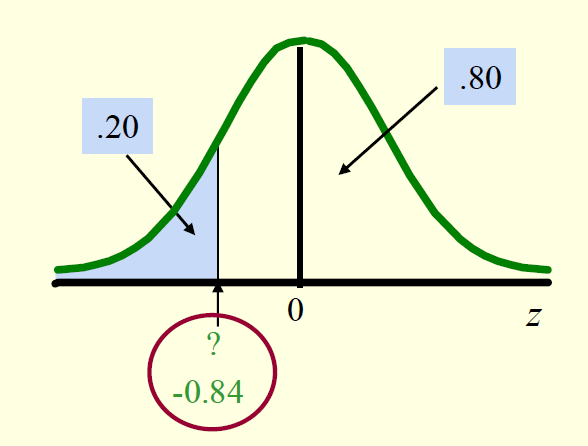
\includegraphics[width=0.6\textwidth]{image_2.png}
  \caption{$20\%$ of the area is before $z = -0.84$}
  \label{fig:finding-z-value}
\end{figure}


\begin{figure}[h!]
  \centering
  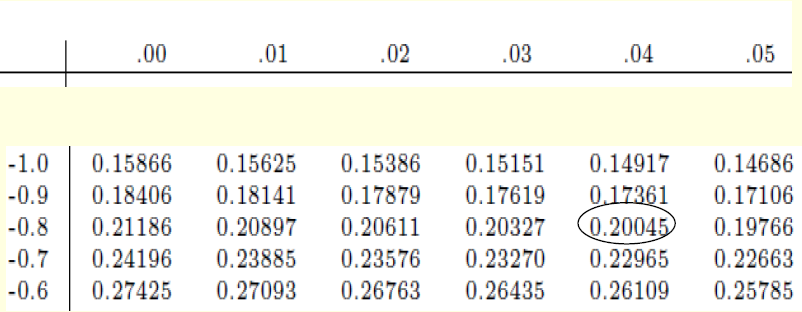
\includegraphics[width=0.8\textwidth]{image_3.png}
  \caption{}
  \label{fig:z-value-table}
\end{figure}
\end{itemize}

\newpage
\section{Chi-squared distributions}

\textbf{Definition 1.} 
Let $X_1, X_2, \dots, X_n$ be independent random variables with $N(0,1)$ distribution. Then for the random variable
\[ \boxed{Y = X_{1}^{2} + X_{2}^{2} + \dots + X_{n}^{2}} \]
it is said that $Y$ has a \textbf{chi-square distribution} with \textbf{$n$ degrees of freedom}, and it is written as $Y \sim \chi^2_n$. 

According to the definition, if $n = 1$, $Y = X^2$ has a chi-square distribution with 1 degree of freedom, if $X \sim N(0,1)$. We write $Y \sim \chi^2_1$.

For the mean and variance of a chi-square distribution with $n$ degrees of freedom, we have:

\[ E(\chi_{n}^2) = (\frac{n}{2})\cdot 2 = n \]
\[ D(\chi_{n}^2) = (\frac{n}{2}) \cdot 2^2 = 2n \]

If the random variable $X \sim N(\mu, \sigma^2)$ then the random variable

\[ Y = \frac{X - \mu}{\sigma} \sim N(0,1) \]

According to the previously statements, the random variable

\[ Y^2 = \frac{(X - \mu)^2}{\sigma^2} \sim \chi_1^2 \]

\subsection{Graphical representation of Chi-squared distribution for $df=3,5,10$}

The Figure \ref{fig:chi} shows the density graphs of the $\chi^2$ distribution with 3, 5, and 10 degrees of freedom.

It can be observed that the peak of the density function decreases as the value of the parameter increases and shifts to the right.


\begin{figure}[h!]
  \centering
  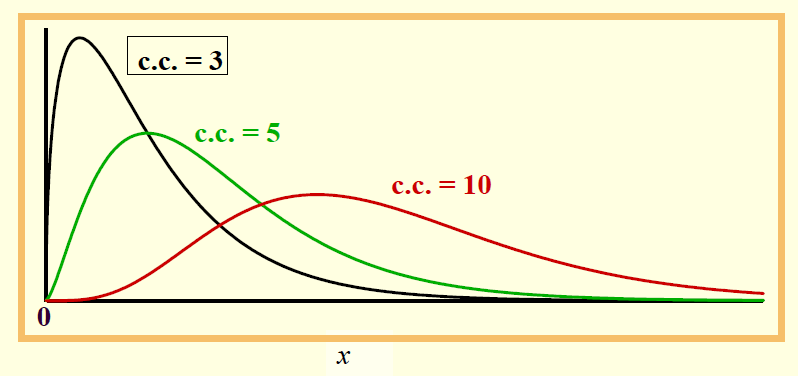
\includegraphics[width=0.6\textwidth]{image_4.png}
  \caption{Chi-squared distribution with degrees of freedom 3,5 and 10}
  \label{fig:chi}
  
\end{figure}

\subsection{Tables for Chi-squared distribution}

From the table, for a given number of degrees of freedom $\nu$ and a given $\alpha$, the value $\chi^2_{\alpha, \nu}$ is read such that

\[ P \{ \chi^2 > \chi_{\alpha, \nu}^{2} \} = \alpha \]

\begin{figure}[h!]
  \centering
  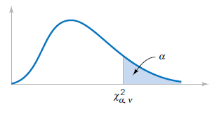
\includegraphics[width=0.4\textwidth]{image_5.png}
  \caption{}
  \label{fig:example_image}
\end{figure}

\begin{figure}[h!]
  \centering
  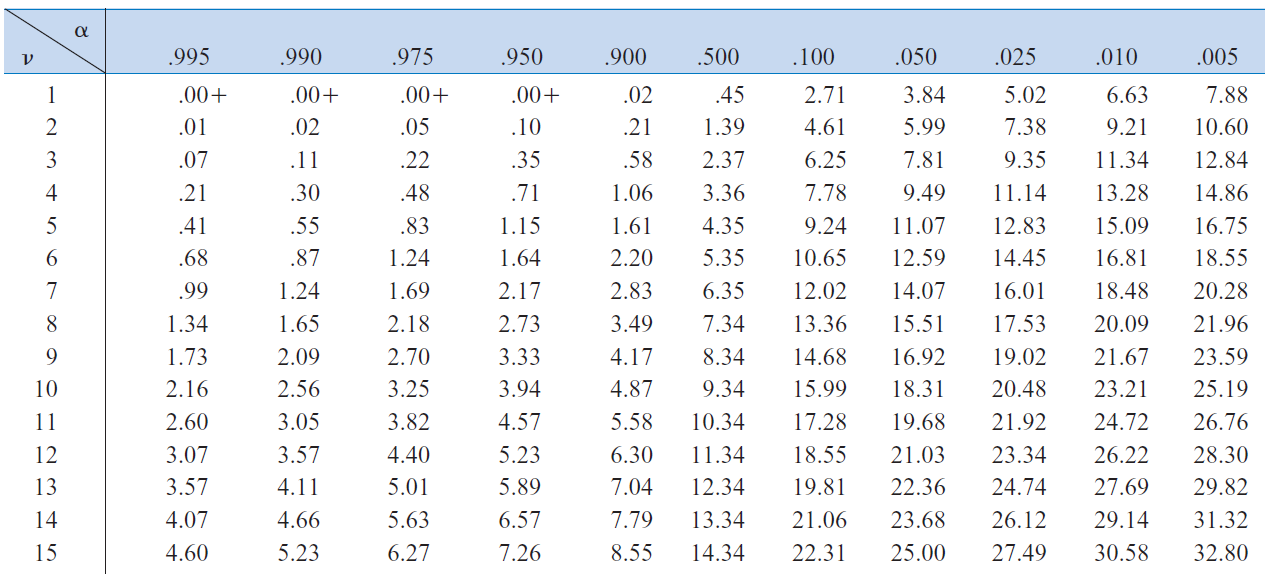
\includegraphics[width=0.8\textwidth]{image_6.png}
  \caption{}
  \label{fig:example_image}
\end{figure}

\subsubsection{Reading from Chi-square table}

Let the random variable $X \sim \chi^2_7$ and we want to determine the value $x$ such that $P\{X > x\} = 0.025.$ Then $x = \chi^2_{0.025,7} = 16.01$.


\begin{figure}[h!]
  \centering
  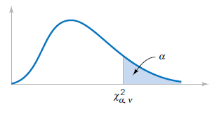
\includegraphics[width=0.4\textwidth]{image_7.png}
  \caption{}
  \label{fig:example_image}
\end{figure}


\begin{figure}[h!]
  \centering
  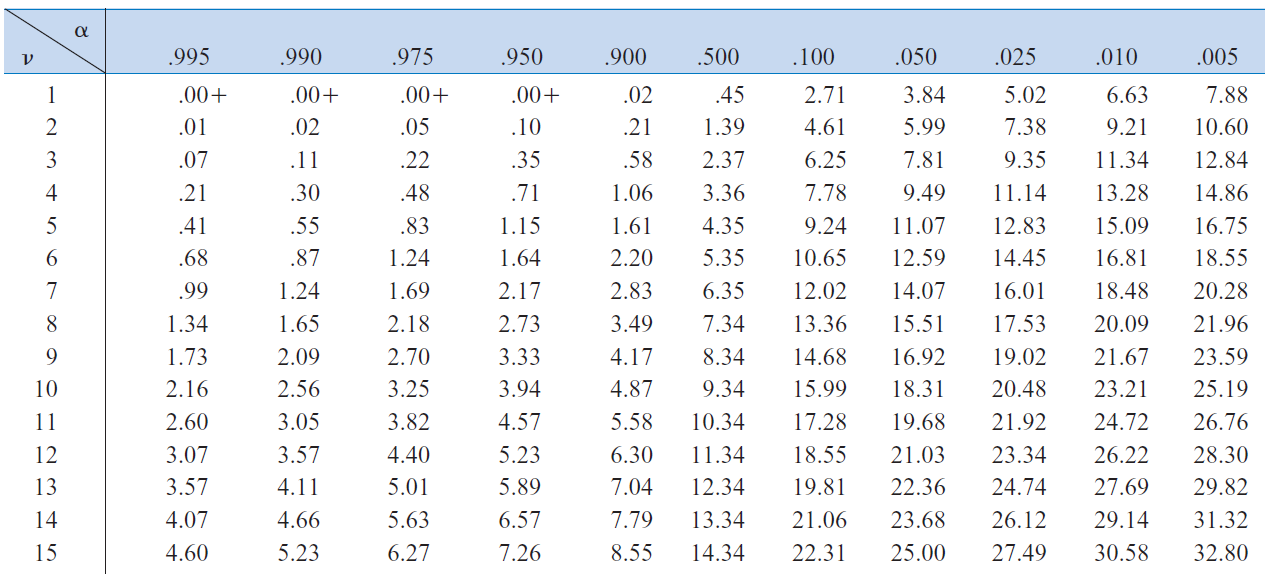
\includegraphics[width=0.8\textwidth]{image_8.png}
  \caption{}
  \label{fig:example_image}
\end{figure}

\section{Student or $t$-distribution}

If $X$ and $Y$ are independent random variables, where $X$ has a standard normal distribution, $X \sim N(0,1)$, and $Y$ has a chi-square distribution with $n$ degrees of freedom, $Y \sim \chi^2_n$, then the distribution of the random variable


\[\boxed{T = \frac{X}{\sqrt{Y/n}}}\]


is known as the Student's $t$-distribution with $n$ degrees of freedom, and it is denoted as $T \sim t_n$.

That is:

\[ \frac{N(0,1)}{\sqrt{\frac{\chi_n^2}{n}}} \sim t_n \]

Thus, the $t$-distribution depends on a single parameter, which is called the number of degrees of freedom.\\

The range of values of this random variable is $(-\infty, +\infty)$.

\begin{figure}[h!]
  \centering
  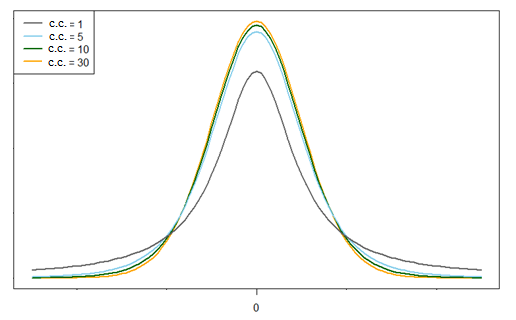
\includegraphics[width=0.8\textwidth]{image_9.png}
  \caption{}
  \label{fig:example_image}
\end{figure}

There is a table for the $t$-distribution, and from it, for a given number of degrees of freedom $\nu$ and a given $\alpha$, the value $t_{\alpha, \nu}$ is read such that

\[P\{T > t_{\alpha, \nu}\} = \alpha\]

Similarly to the $\chi^2$ distribution, from the tables for the $t$-distribution, for a given number of degrees of freedom $\nu$ and a given $\alpha$, the value $t_{\alpha, \nu}$ is read such that

\[
P\{T > t_{\alpha, \nu}\} = \alpha.
\]

\begin{figure}[h!]
  \centering
  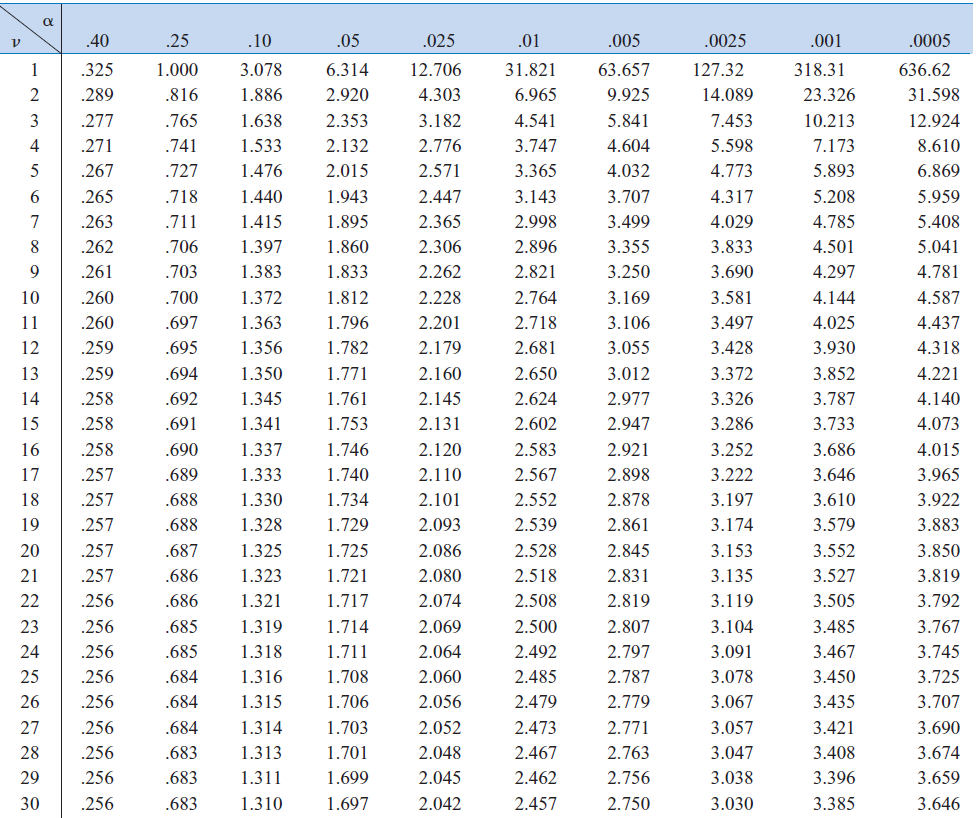
\includegraphics[width=0.8\textwidth]{image_10.png}
  \caption{}
  \label{fig:example_image}
\end{figure}

\begin{figure}[h!]
  \centering
  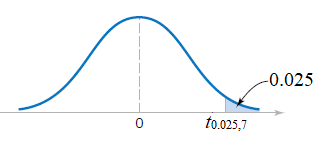
\includegraphics[width=0.4\textwidth]{image_11.png}
  \caption{$t_{0.0.5,7} = 2.365$}
  \label{fig:example_image}
\end{figure}

\begin{figure}[h!]
  \centering
  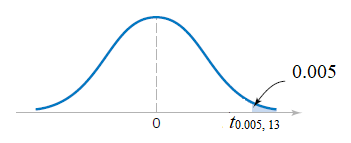
\includegraphics[width=0.4\textwidth]{image_12.png}
  \caption{$t_{0.005,13} = 3.012$}
  \label{fig:example_image}
\end{figure}



If it is given that $T \sim t_{18}$, the question is how to determine the value $x$ such that

\[ P\{T > x\} = 0.25 \]

According to the tabulated values in the $t$-distribution table,

\[x = t_{0.25, 18} = 0.688. \]

\begin{figure}[h!]
  \centering
  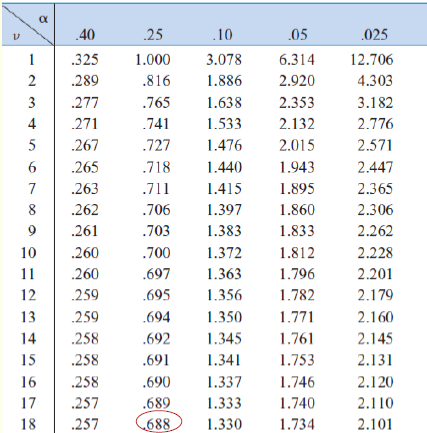
\includegraphics[width=0.4\textwidth]{image_13.png}
  \caption{}
  \label{fig:example_image}
\end{figure}


\begin{figure}[h!]
  \centering
  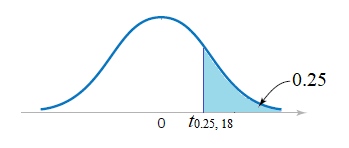
\includegraphics[width=0.4\textwidth]{image_14.png}
  \caption{}
  \label{fig:example_image}
\end{figure}


It can be observed that as the number of degrees of freedom increases, the density graphs of the $t$-distribution increasingly approach the graph of the standard normal distribution.\\

The approximation is considered good if $n > 30$.

\begin{figure}[h!]
  \centering
  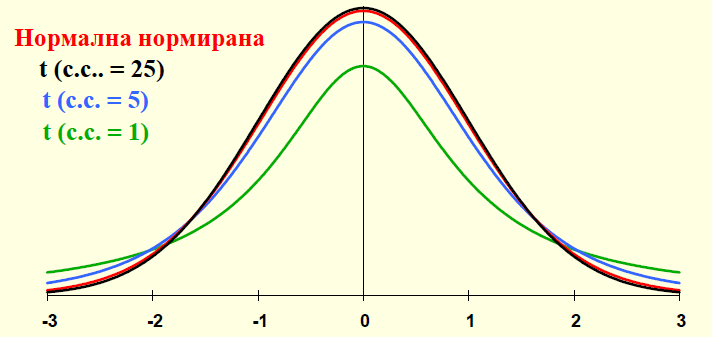
\includegraphics[width=0.6\textwidth]{image_15.png}
  \caption{}
  \label{fig:t-to-standard-normal}
\end{figure}



\newpage 
\subsubsection{Comparison of t-distribution and standard normal distribution}

If it is given that $T \sim t_{45}$, and we need to determine the value $x$ such that $P\{T > x\} = 0.25$ , then we use the relationship between the $t$-distribution and the standard normal distribution.

Therefore,
\[
P\{T > x\} \approx P\{Z > x\} = 0.25, \quad \text{i.e., } P\{Z < x\} = 0.75.
\]

Now, in the standard normal distribution table, we look for the value 0.75 (or the closest to it). We obtain $x = 0.66$.

\section{Fisher or $F$-distribution}

The Fisher distribution is obtained when the ratio of two independent chi-square random variables is divided by their respective degrees of freedom.\\

If $X \sim \chi^2_{n_1}$ and $Y \sim \chi^2_{n_2}$ are independent random variables, then the random variable

\[ \boxed{F = \frac{X / n_1}{Y / n_2}} \]

has a Fisher distribution with $n_1$ and $n_2$ degrees of freedom. It is denoted as $F \sim F_{n_1, n_2}$. \\

The number $n_1$ is called the numerator degrees of freedom, and the number $n_2$ is called the denominator degrees of freedom. \\

The $F$-distribution is an absolutely continuous distribution that depends on two parameters, which are called the number of degrees of freedom. \\ 

The range of values of this random variable is $(0, +\infty)$.


\begin{figure}[h!]
  \centering
  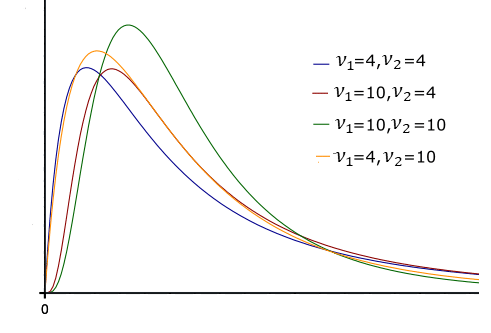
\includegraphics[width=0.6\textwidth]{image_16.png}
  \caption{Fisher distribution}
  \label{fig:fisher-distr}
\end{figure}

There are tables for the $F$-distribution from which, for given degrees of freedom $\nu_1$ and $\nu_2$ and a given $\alpha$, the value $f_{\alpha, \nu_1, \nu_2}$ is read such that

\[ P\{F > f_{\alpha, \nu_1, \nu_2}\} = \alpha\]

where $F$ is a random variable that has an $F_{\nu_1, \nu_2}$ distribution.


\begin{figure}[h!]
  \centering
  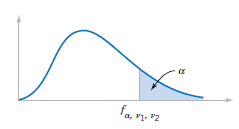
\includegraphics[width=0.6\textwidth]{image_17.png}
  \caption{}
  \label{fig:example_image}
\end{figure}

\subsection{Table for $F$-distribution for $\alpha = 0.025$}

\[ f_{0.025, 10,5} = 6.62\] 

\subsection{Table for $F$-distribution for $\alpha = 0.05$}

\[ f_{0.025, 5,10} = 3.33\]

The problem with these tables is that they exist only for a few (mainly smaller) values of $\alpha$, so if we need to read the value for some other $\alpha$, it cannot be done directly.\\

However, the following equality for the values of $F$-distributions can be used. Namely,

\[
f_{1 - \alpha, \nu_1, \nu_2} = \frac{1}{f_{\alpha, \nu_2, \nu_1}}.
\]

Example: Table for $F$-distribution for $\alpha = 0.05$

\[
f_{0.95, 10, 15} = \frac{1}{f_{0.05, 15, 10}} = \frac{1}{2.85} = 0.35.
\]


\end{document}